% compile with XeLaTeX or LuaLaTeX

\documentclass[a4paper,12pt]{article} %14pt - extarticle
\usepackage[utf8]{inputenc} % russian, do not change
\usepackage[T2A, T1]{fontenc} % russian, do not change
\usepackage[english, russian]{babel} % russian, do not change

% fonts
\usepackage{fontspec} % different fonts
\setmainfont{Times New Roman}
\usepackage{setspace,amsmath}
\usepackage{amssymb} %common math symbols
\usepackage{dsfont}

% utilities
\usepackage{graphicx}
\usepackage{float} % force pictures position with [H]
\usepackage{hyperref}
\hypersetup{pdfstartview=FitH,  linkcolor=blue, urlcolor=blue, colorlinks=true}

% misc
\graphicspath{{./img/}}

\begin{document}
	
\section{14. FASTA}
Алгоритм FASTA (от англ. 'fast-all'; 'all' означает, что программа работает с любым языком -- хоть нуклеотидным, хоть белковым): ищет локальные выравнивания с высокой стоимостью между последовательностью и базой. Сейчас чаще используется более новый алгоритм BLAST.

Говорят, что пара якорей $(i_1,j_1), (i_2, j_2)$ \textit{принадлежит одной диагонали}, если $i_1-j_1=i_2-j_2$.

\begin{figure}[H]
	\centering 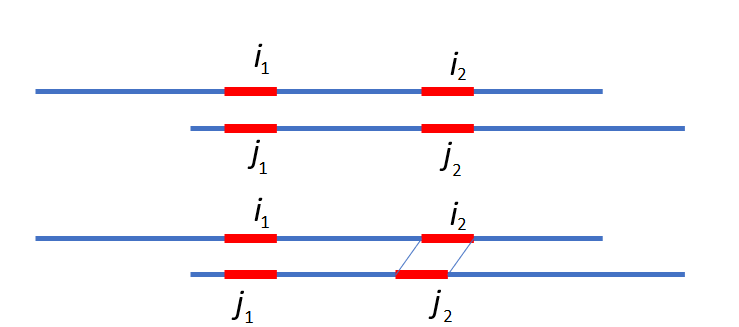
\includegraphics[width=.6\textwidth]{seeds}
	\caption{Вверху: пара якорей $(i_1,j_1), (i_2, j_2)$ на одной диагонали; внизу -- не на одной диагонали}
\end{figure}

\textit{Мощностью} диагонали назовём число якорей на ней.

Алгоритм отбирает $n$ самых мощных диагоналей (обычно $n=10$), после чего методом локального динамического программирования строится выравнивание в полосе около каждой из них.

\subsection{Дополнительная информация}
Q: Как выбрать длину l-грамы для поиска якорей? \\
A: Больше значение l \textrightarrow больше скорость поиска, но меньше чувствительность (меньше якорей найдём), и наоборот. Для нуклеотидных последовательностей обычно $l \approx 4-6$, для белковых 2. Чтобы чувствительность была сравнима с таковой для алгоритмов динамического программирования, нужно брать $l=1$.

Ссылки:\\
\href{https://www.youtube.com/watch?v=gGoYQBBEX8M&list=PLvJPYisgz4MDD0mcjf9HBu9OX-gb-7WZc&t=1004s}{YouTube: лекция 2, 16:44}\\
Презентация: \href{https://vk.com/doc155237002_519204981?hash=85ffc7a5b3eb31882d}{lecture3.pdf}

\section{44. Функция правдоподобия, оценка максимального правдоподобия}

Пусть есть предсказывающая модель $M$ с набором параметров $\vartheta$ и набор данных $D$ (например, $M$ -- нормальное распределение, $\vartheta = {\mu, \sigma}$, $D$ -- набор точек ${(x_i, y_i)}$, сгенерированных по нормальному закону). Хотим наилучшим образом подогнать модель под набор данных.

Очевидная стратегия -- максимизируем вероятность набора данных $D$ при условии выбора параметров $\theta$, т. е. ищем
$$\theta^* = \arg \max_{\theta}P(D|\theta, M)$$

Вообще, $P(x|y)$ как функция $x$ -- \textit{вероятность} (данных при условии параметров), а как функция $y$ -- \textit{правдоподобие} (параметров при условии данных).

Пусть данные $D = \{(x_i, y_i)\}$. Конечно же, мы считаем, что точки сгенерированы независимо. Тогда
$$P(D|\theta, M) = \prod_{i}P((x_i, y_i)|\theta, M)$$
Удобно перейти к логарифмам:
$$\theta^* = \arg \max_\theta \sum_{i} \log P((x_i, y_i) | \theta, M)$$

\subsection{Дополнительная информация}
Оценка максимального правдоподобия обладает свойством \textit{состоятельности}: если взять модель с параметрами $\theta_0$ и сгенерировать набор $D$ данных, то в пределе $\theta^* \xrightarrow[|D| \to \infty]{} \theta_0$.

Минус метода -- если данных недостаточно, результат может сильно отличаться от реальности. В таких случаях надо искать дополнительную априорную информацию (например, при расчёте вероятностей выпадения граней у кости в нечестном казино можно априорно постановить, что каждая близка к $\frac{1}{6}$).

Подробнее: Дурбин, \textsection 11.3 Статистическая оценка параметров / Максимальное правдоподобие. \\
YouTube: всё это относится к лекции 5; слайды -- \href{https://vk.com/doc155237002_582644273?hash=fb93b84e1043bdc4db}{лекция 6}. Но там нет нигде отдельно чётко про функцию правдоподобия, лучше см. Дурбина.

\section{60. Выравнивание последовательности относительно профиля СММ семейства}
Вопросы 60-61: \href{https://www.youtube.com/watch?v=HD_VI41SmV4&list=PLvJPYisgz4MDD0mcjf9HBu9OX-gb-7WZc&t=2584s}{YouTube: лекция 2, 43:04}


Как выровнять последовательность относительно профиля данной СММ? Задача решается с помощью адаптированного алгоритма Витерби. Результат сравнения в ячейке матрицы динамического программирования -- \textit{log-odds ratio} вероятности неслучайного выравнивания к вероятности случайного (подробнее про log-odds ratio см. вопрос  2, "матрицы замен")

Пусть $V_j^M(i)$ -- оценка логарифма отношения правдоподобия для пути с наилучшим сходством между подпоследовательностью $x_i$ и подмоделью до состояния с номером $j$ при условии, что в последней позиции match (совпадение); $V_j^I(i)$ -- та же оценка, но в последней позиции инсерция; $V_j^I(i)$ -- в последней позиции делеция. Тогда
\begin{multline*}
	\cr	V_j^M(i) = \log \frac{e_{M_j}(x_i)}{q_{x_i}} + \max \left\{
	\begin{array}{ll}
		V_{j-1}^M(i-1) + \log a_{M_{j-1}M_j}\\
		V_{j-1}^I(i-1) + \log a_{I_{j-1}M_j}\\
		V_{j-1}^D(i-1) + \log a_{D_{j-1}M_j}
	\end{array}
	\right. \\
	\cr	V_j^I(i) = \log \frac{e_{I_j}(x_i)}{q_{x_i}} + \max \left\{
	\begin{array}{ll}
		V_{j}^M(i-1) + \log a_{M_{j}I_j}\\
		V_{j}^I(i-1) + \log a_{I_{j}I_j}\\
		V_{j}^D(i-1) + \log a_{D_{j}I_j}
	\end{array}
	\right. \\
	\cr	V_j^D(i) = \max \left\{
	\begin{array}{ll}
		V_{j-1}^M(i) + \log a_{M_{j-1}D_j}\\
		V_{j-1}^I(i) + \log a_{I_{j-1}D_j}\\
		V_{j-1}^D(i) + \log a_{D_{j-1}D_j}
	\end{array}
	\right. \\
\end{multline*}

\subsection{Дополнительная информация}

Если вероятность эмиссии в состоянии инсерции считаем равной фоновой вероятности, то в формуле для $V_j^I(i)$ первое слагаемое, где логарифм дроби, можно убрать. Также можно считать, что переходы D->I и I->D не реализуются (то есть после делеции или инсерции будет непременно хотя бы один match, иначе выравнивание очень странное), и убрать их из расчёта максимума.

\section{61. Как определить вероятность того, что последовательность может быть порождена данной СММ}
Используется прямой алгоритм. Значение в каждой клетке -- log-odds ratio вероятности того, что последовательность порождена данной СММ к вероятности случайного сходства (почти как в алгоритме Витерби из вопроса 60).


\section{65 Множественное выравнивание относительно известного профиля СММ}

Вопросы 65-66: Дурбин, \textsection 6.5 Множественное выравнивание. стр. 208. Множественное выравнивание с известной СММ.\\
\href{https://youtu.be/HD_VI41SmV4?t=2957}{YouTube: лекция 2, 49:17}


Пусть у нас есть готовое множественное выравнивание. На его основании можно построить профильную СММ. После этого, применяя алгоритм Витерби, можно найти выравнивание новой последовательности к этой СММ. Можно сказать, что новая последовательность «подравнивается» к старым (старое выравнивание при этом остаётся неизменным).

\section{66 Множественное выравнивание, когда профиль СММ неизвестен}

Можно обучать профильные HMM, начиная с невыровненных последовательностей, используя алгоритм максимизации ожидания (Expectation Maximization) Баума-Уэлча:
\begin{enumerate}
	\item Порождаем случайные параметры СММ (E-шаг)
	\item Выравниваем все последовательности
	\item Переоцениваем параметры (M-шаг)
\end{enumerate}

В итоге в итерациях мы приблизимся к правильному выравниванию. Но алгоритм медленно сходится (как и всегда с алгоритмом Баума-Уэлча).

\section{77. Поиск общего мотива}
\href{https://www.youtube.com/watch?v=zR9ZRMmMdY0&list=PLvJPYisgz4MDD0mcjf9HBu9OX-gb-7WZc&t=3993s}{YouTube: лекция 8, 1:06:33}\\
Презентация: \href{https://vk.com/doc155237002_582644476?hash=d8a8032e4fcc7c9f4d}{motif8\_9.pptx} (слайды 46-48 из 83)

Задача: есть группа генов, о которых мы предполагаем, что они регулируются общим ТФ, но о самом ТФ ничего не знаем. Нужно найти мотив (сайт присоединения ТФ), общий для нескольких последовательностей. Похожая задача -- поиск CpG-островков.

\begin{figure}[H]
	\centering 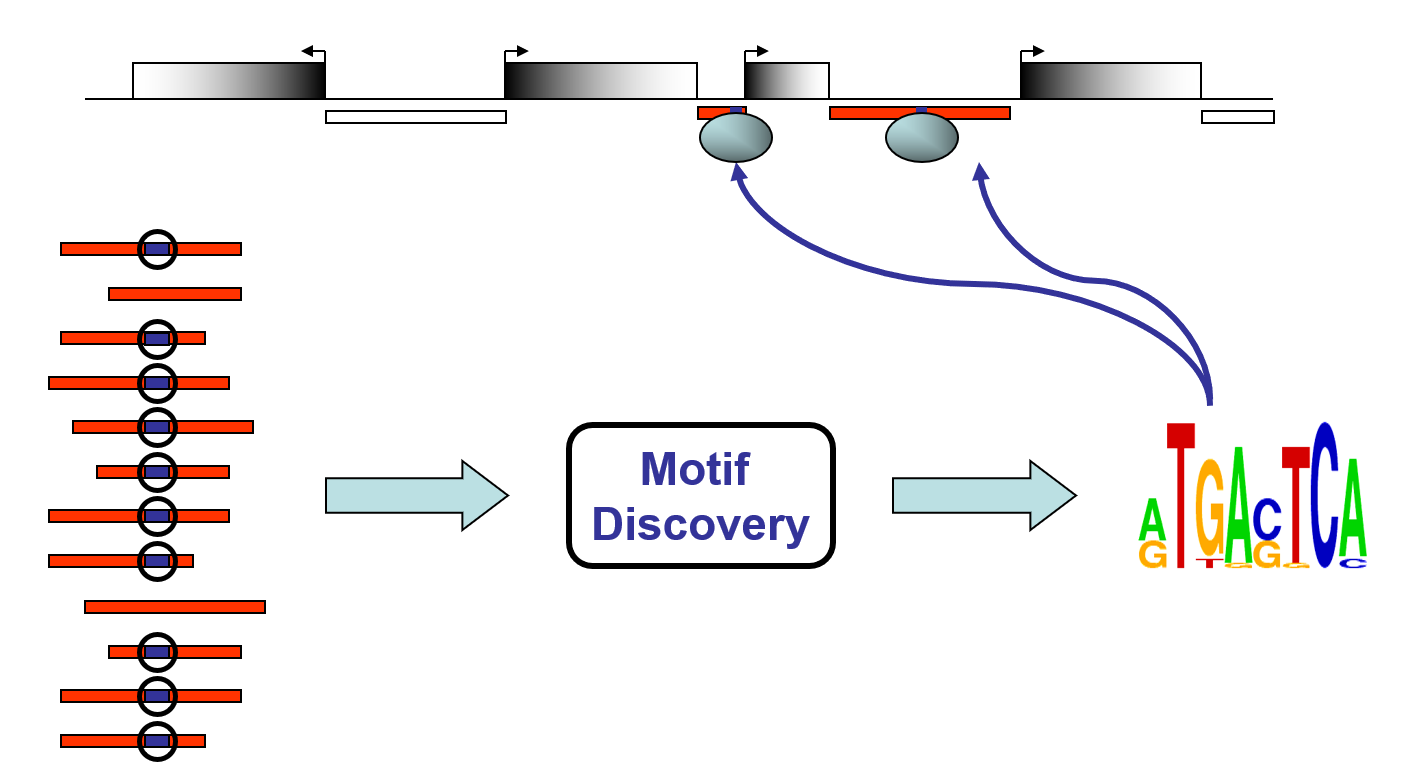
\includegraphics[width=.8\textwidth]{motif_discovery}
\end{figure}

Возможные методы решения (подробно разобраны в вопросах 78-83):
\begin{itemize}
	\item Вероятностные методы - СММ, ЕМ, Gibbs Sampling...
	\item Последовательный перебор: очень трудоёмко, особенно для длинных мотивов и при их неполном совпадении (а мы помним, что мотивы отличаются высокой вариабельностью и чаще не совпадают, чем совпадают)
	\item Использование дополнительной информации о последовательностях: филогения, кластеризация...
	\item Учёт конформационных свойств ДНК
\end{itemize}

\end{document}